\documentclass{./../div_teaching_slides}

\begin{document}
\title{ECON 340 \\ Economic Research Methods}
\author{Div Bhagia}
\date{Lecture 12: Good Estimators, Sample Mean Distribution, Confidence Intervals}

%%%%%%%%%%%% 
\begin{frame}[noframenumbering, plain]
\maketitle
\end{frame}

%%%%%%%%%%%% 
\begin{frame}{Sampling and Estimation}
\begin{witemize}
\item We want to learn something about the population
\item But often, we can collect data only for a sample of the population
\item Good news: if the sample is drawn \textit{randomly} we can use statistical methods to reach \textit{tentative} answers 
\item Use sample quantities to \textit{estimate} population parameters
\item Sample \textit{estimators} are random variables
\end{witemize}
\end{frame}

%%%%%%%%%%%%
\begin{frame}{Estimators}
\begin{witemize}
  \item Denote the population parameter of interest by $\theta$
  \item And let's denote its sample estimator by $\hat{\theta}$
  \item Three desirable properties for an estimator: \\
  \begin{witemize}
  \normalsize
  \item \textit{Unbiasedness}: $ E(\hat{\theta}) = \theta $
  \item \textit{Efficiency}: lower variance is better
  \item \textit{Consistency}: as the sample size becomes infinitely large,  $\hat{\theta} \rightarrow \theta$
\end{witemize}
\end{witemize}
\end{frame}

%%%%%%%%%%%%
\begin{frame}{What is a good estimator?}
\centering
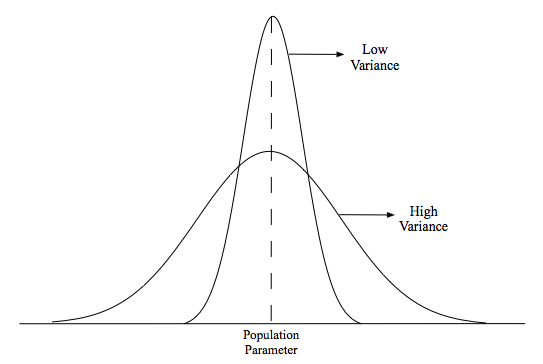
\includegraphics[scale=0.6]{effeciency.png}
\end{frame}


%%%%%%%%%%%%
\begin{frame}{Expectation and Variance of $\bar{X}$}
Let $X_1,X_2,...,X_n$ denote independent random draws (random sample) from a population with mean $\mu$ and variance $\sigma^2$. 
$$ \bar{X} = \frac{1}{n} \sum_{i=1}^n X_i $$
Then $\bar{X}$ is also a random variable with:
$$E(\bar{X}) = \mu \quad \quad  Var(\bar{X}) = \frac{\sigma^2}{n} $$ 

So $\bar{X}$ is an unbiased and consistent estimator for $\mu$.
\end{frame}

%%%%%%%%%%%%
\begin{frame}{Sample Mean Distribution}
The distribution of the sample mean is \underline{normal} if \textit{either} of the following is true: \\~\\
\begin{witemize}
  \item The underlying population is normal
  \item The sample size is large, say $n\geq 100$ \\~\\
\end{witemize}
The first one follows from the sample mean being a linear combination of normally distributed variables. \\~\\

The latter is implied by the \textit{Central Limit Theorem}. 
\end{frame}

%%%%%%%%%%%%
\begin{frame}{Central Limit Theorem}
\vspace{2em}
If $X_1, X_2,..,X_n$ are drawn randomly from a population with mean $\mu$ and variance $\sigma^2$, sample mean $\bar{X}$ is normally distributed with mean $\mu$ and variance $\sigma^2/n$ as long as $n$ is large.
$$\bar{X} \sim N\left(\mu, \dfrac{\sigma^2}{n}\right)$$ \\~\\
\href{https://dbhagia.shinyapps.io/CLT-Demo/}{\blue{Simulation}}
\end{frame}

%%%%%%%%%%%%
\begin{frame}{Normal Population}
\centering
\begin{columns}
\begin{column}{0.475\textwidth}
\centering
Normal Population \\ $\mu=5, \sigma^2 = 9$ \\~\\
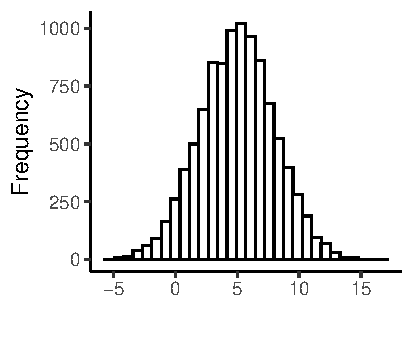
\includegraphics{./../../output/clt_norm_pop.pdf}
\end{column}
\begin{column}{0.475\textwidth}
\centering
Sample Mean Distribution \\ $n=10, E(\bar{X})=5, Var(\bar{X}) = 0.9$ \\~\\
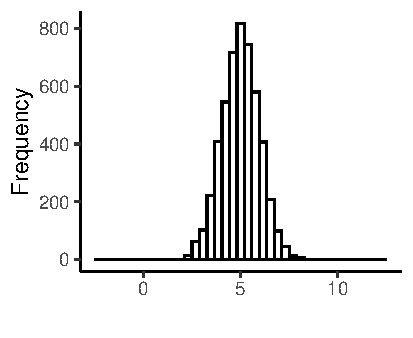
\includegraphics{./../../output/clt_norm_samp_n10.pdf}
\end{column}
\end{columns}
\end{frame}

%%%%%%%%%%%%
\begin{frame}{Non-Normal Population}
\centering
\begin{columns}
\begin{column}{0.475\textwidth}
\centering
Non-Normal Population \\ $\mu=1, \sigma^2 = 1$ \\~\\
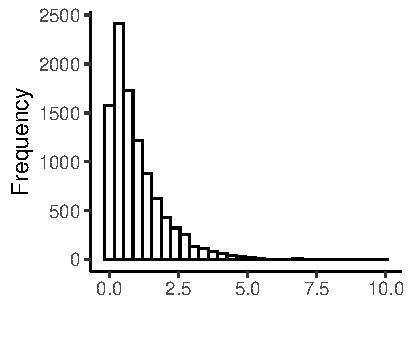
\includegraphics{./../../output/clt_exp_pop.pdf}
\end{column}
\hspace{-2em}
\begin{column}{0.55\textwidth}
\centering
Sample Mean Distribution \\ $n=10, E(\bar{X})=0.92, Var(\bar{X}) = 0.1$ \\~\\
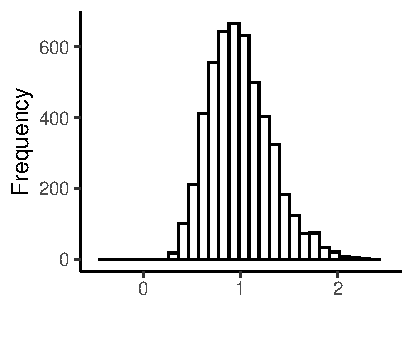
\includegraphics{./../../output/clt_exp_samp_n10.pdf}
\end{column}
\end{columns}
\end{frame}

%%%%%%%%%%%%
\begin{frame}{Central Limit Theorem}
\centering
\begin{columns}
\begin{column}{0.475\textwidth}
\centering
Non-Normal Population \\ $\mu=1, \sigma^2 = 1$ \\~\\
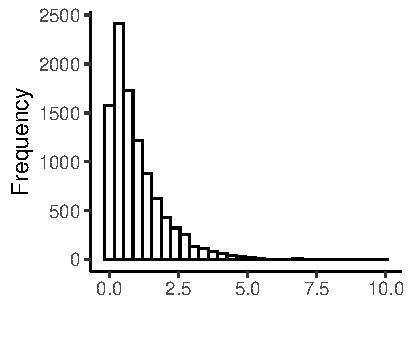
\includegraphics{./../../output/clt_exp_pop.pdf}
\end{column}
\begin{column}{0.475\textwidth}
\centering
Sample Mean Distribution \\ $n=100, \bar{X}=1, Var(\bar{X}) = 0.01$ \\~\\
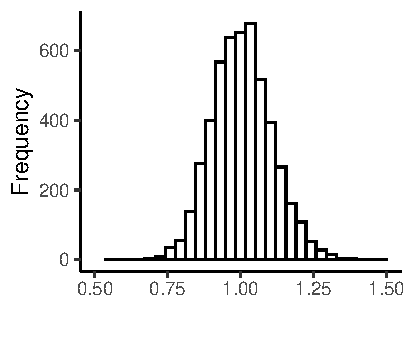
\includegraphics{./../../output/clt_exp_samp_n100.pdf}
\end{column}
\end{columns}
\end{frame}

%%%%%%%%%%%%
\begin{frame}{Example: Blood Pressure in Massachusetts}
\centering \vspace{-0.5em}
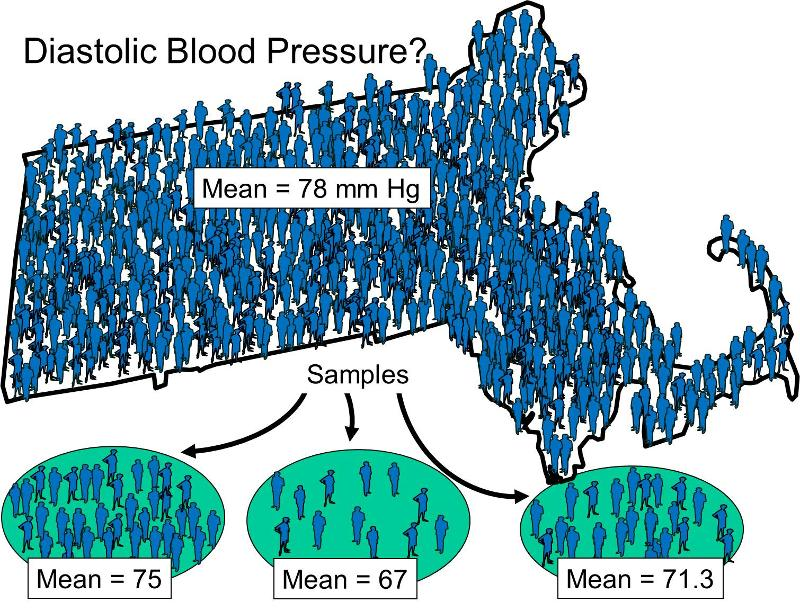
\includegraphics[scale=0.35]{Sampling3.jpg}
\end{frame}

%%%%%%%%%%%%
\begin{frame}{Confidence Intervals}
\begin{witemize}
	\item Let's say we picked a random sample of 100 people from Massachusetts and took their blood pressure and found $\bar{x} = 75$. 
  \item Given this estimate of 75, what can we say about the true mean?
  \item Here $n=100$ so by CLT, $\bar{X} \sim N(\mu, \sigma^2/n) $. For now assume we know $\sigma^2=552.25$.
  \item Then we should be able to say with some certainty that the true mean lies \textit{somewhere} around 75.
\end{witemize}
\end{frame}


%%%%%%%%%%%%
\begin{frame}{Confidence Intervals}
\begin{witemize}
  \item Create an interval around the sample mean that gives us a range of plausible values for the population mean.
  \item We can have confidence intervals of varying levels of confidence, most common are 90\%, 95\%, or 99\%.
  \item The level of confidence is the probability that a calculated confidence interval contains the true population parameter. 
  \end{witemize}
\end{frame}


%%%%%%%%%%%%
\begin{frame}{How to construct a confidence interval?}
Say we want to construct a 90\% confidence interval for the true mean.\\~\\
So far we have established that $\bar{X} \sim N(\mu, \sigma^2/n) $. \\~\\

Note that then,
$$ Z = \frac{\bar{X}-\mu}{\sigma_{\bar{X}}} = \frac{\bar{X}-\mu}{\sigma/\sqrt{n}} \sim N(0,1)$$ \vspace{0.5em}

From the Standard Normal table, we can find that 
 $$ P(-1.64 < Z < 1.64) = 0.90 $$
\end{frame}

%%%%%%%%%%%%
\begin{frame}{Standard Normal Distribution}
\vspace{1em} \centering
\begin{tikzpicture}
\begin{axis}[
  no markers, domain=-3:3, samples=100,
  axis lines*=left, xlabel=Z, ylabel=$f(Z)$,
  %every axis y label/.style={at=(current axis.above origin),anchor=south},
  height=6.5cm, width=12cm,
  xtick={-1.64, 0, 1.64}, %ytick=\empty,
  enlargelimits=false, clip=false, axis on top,
  ]
  \addplot [very thick,black] {gauss(0, 1)}; 
  \addplot [fill=purple!20, draw=none, domain=-1.64:1.64] {gauss(0, 1)} \closedcycle;
%\draw[->, line width=1pt](axis cs: 185, 0.0125)--(axis cs: 205, 0.0125);
\node at (axis cs: 0, 0.2) {90\%};
\end{axis}
\end{tikzpicture}
\end{frame}

%%%%%%%%%%%%
\begin{frame}{Normal Distribution}
90\% of the area under the curve lies within 1.64 standard deviations of the mean. 
\vspace{1em} 

\centering
\begin{tikzpicture}
\begin{axis}[
  no markers, domain=-3:3, samples=100,
  axis lines*=left, xlabel=X, ylabel=$f(X)$,
  %every axis y label/.style={at=(current axis.above origin),anchor=south},
  height=6cm, width=12cm,
  xtick={-1.64, 0, 1.64}, xticklabels={$\mu-1.64 \sigma_X$, $\mu$, $\mu+1.64 \sigma_X$}, %ytick=\empty,
  enlargelimits=false, clip=false, axis on top,
  ]
  \addplot [very thick,black] {gauss(0, 1)}; 
  \addplot [fill=purple!20, draw=none, domain=-1.64:1.64] {gauss(0, 1)} \closedcycle;
%\draw[->, line width=1pt](axis cs: 185, 0.0125)--(axis cs: 205, 0.0125);
\node at (axis cs: 0, 0.2) { 90\%};
\end{axis}
\end{tikzpicture} \\
\end{frame}



%%%%%%%%%%%%
\begin{frame}{90\% Confidence Intervals}
 $$ Pr(-1.64 < Z < 1.64) = 0.90 $$ \\
 $$ Pr\left(-1.64 < \frac{\bar{X}-\mu}{\sigma_{\bar{X}}} < 1.64 \right) = 0.90 $$ \\
   $$ Pr\left( \mu -1.64 \sigma_{\bar{X}} < \bar{X}<   \mu+  1.64 \sigma_{\bar{X}} \right) = 0.90 $$ \\
  $$ Pr\left( \bar{X} -1.64 \sigma_{\bar{X}} < \mu <   \bar{X}+  1.64 \sigma_{\bar{X}} \right) = 0.90 $$
\end{frame}

%%%%%%%%%%%%
\begin{frame}{90\% Confidence Intervals}
$$ Pr\left( \bar{X} -1.64 \sigma_{\bar{X}} < \mu <   \bar{X}+  1.64 \sigma_{\bar{X}} \right) = 0.90 $$ \\ \vspace{1em}
 Note that $\sigma_{\bar{X}}=\sigma/\sqrt{n}$, so the 90\% confidence interval here is given by:
 $$ \bar{x} \pm 1.64\cdot   \frac{\sigma}{\sqrt{n}} $$ \\~\\
 Plugging in $\sigma = \sqrt{552.25}$ and $n=100$. We get $[71.15, 78.85]$. 
\end{frame}

%%%%%%%%%%%%
\begin{frame}{Confidence Intervals: Interpretation}
\vfill
There is a 90\% chance that the true population average for blood pressure lies in this interval. \\~\\

What this really means is that if we took 100 random samples from the population and calculated 90\% confidence intervals for each sample, we would expect 90 out of 100 intervals to contain the true population mean.
\vfill
\end{frame}

%%%%%%%%%%%%
\begin{frame}{Confidence Intervals: Interpretation}
\centering
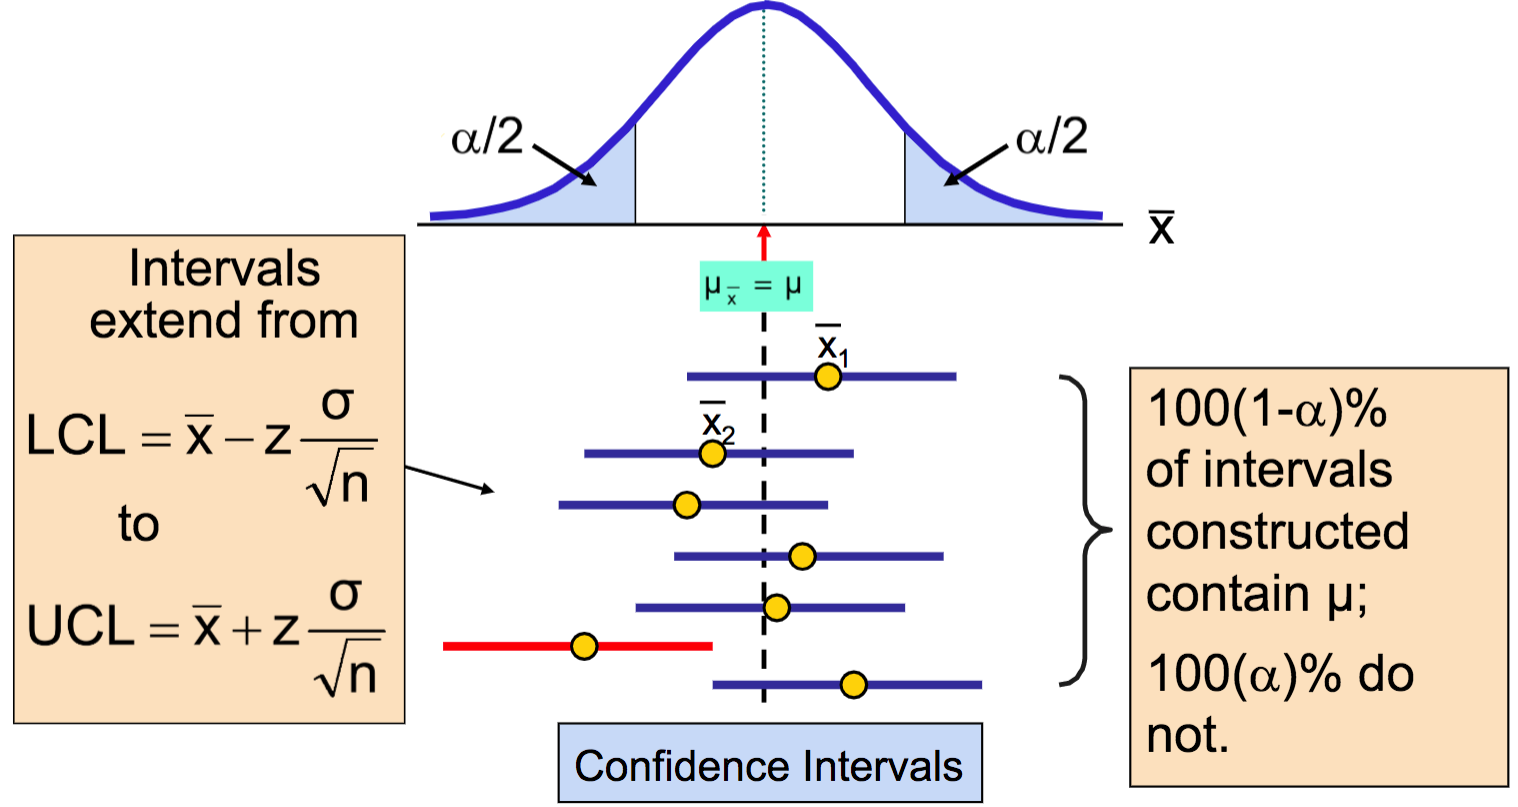
\includegraphics[scale=0.5]{ci_int.png}	
\end{frame}

%%%%%%%%%%%%
\begin{frame}{Confidence Intervals: Recipe}
Let $z_{\alpha/2}$ be the $z$-value that leaves area $\alpha/2$ in the upper tail of the normal distribution. \\~\\
Then $1-\alpha$ confidence interval is given by 
$$ \bar{x} \pm  \underbrace{z_{\alpha/2}  \frac{\sigma}{\sqrt{n}}}_{\text{Margin of Error}} $$
\end{frame}

%%%%%%%%%%%%
\begin{frame}{Next up}
\begin{witemize}
  \item Problem Set 3 is due next Tuesday 
  \item Next week: Continue with sampling and estimation
  \item Week after: Review class and midterm 
\end{witemize}
\end{frame}



\end{document}